\section{Ablation}\label{sec:ablation}

The ablation varies one choice of the method at a time from the reference front (20 weights, 15 steps per weight, a linear schedule, a warm start along the weights, a start from phase-fixed WGS, the scaled loss) on the first \nSeedsAbl{} seeds, and reports the hypervolume of the variant, its paired difference from the reference, the lowest uniformity reached, and the seconds of one thread.
The reference has a hypervolume of \ablDefaultHv{} on these seeds and takes \ablDefaultSec{} seconds in one thread. Table~\ref{tab:ablation} gives the twelve variants and Figure~\ref{fig:ablation} plots the paired differences with their intervals. With five seeds the intervals are wide, and a difference whose interval contains zero is not distinguished from no change.

\subsection{Components of the method}\label{sec:abl-components}

\begin{table}[t]
\centering\small
\caption{Ablation of the front on the ten by ten task: hypervolume of each variant (mean $\pm$ half-width of the 95 percent interval over \nSeedsAbl{} seeds), its paired difference from the reference front, the lowest uniformity on the front and the seconds of one thread. The first row is the reference; every other row changes the one choice named in its first two columns.}
\label{tab:ablation}

\footnotesize\setlength{\tabcolsep}{3pt}
\begin{tabular}{@{}llrrrr@{}}
\toprule
Component & Variant & Hypervolume & Change & Lowest $u$ & Seconds \\
\midrule
Reference & 20 values, 15 steps, linear, warm & $0.8230\pm0.0036$ &  & 0.012 & 64.2 \\
Number of values & 5 values & $0.8130\pm0.0043$ & $-0.0100\pm0.0046$ & 0.015 & 18.7 \\
 & 10 values & $0.8188\pm0.0024$ & $-0.0042\pm0.0034$ & 0.029 & 34.7 \\
 & 40 values & $0.8242\pm0.0031$ & $0.0012\pm0.0017$ & 0.022 & 134.5 \\
Steps per value & 5 steps & $0.8190\pm0.0039$ & $-0.0040\pm0.0043$ & 0.058 & 30.3 \\
 & 30 steps & $0.8235\pm0.0030$ & $0.0005\pm0.0014$ & 0.013 & 118.5 \\
Schedule & quadratic in $\lambda$ & $0.8221\pm0.0036$ & $-0.0009\pm0.0003$ & 0.011 & 70.8 \\
 & target-spaced & $0.8133\pm0.0026$ & $-0.0097\pm0.0012$ & 0.944 & 70.6 \\
Continuation & cold start per value & $0.8134\pm0.0057$ & $-0.0096\pm0.0070$ & 0.020 & 72.7 \\
Start & plain GS start & $0.8170\pm0.0055$ & $-0.0060\pm0.0024$ & 0.019 & 68.2 \\
 & random, no iteration & $0.8143\pm0.0046$ & $-0.0087\pm0.0051$ & 0.012 & 59.8 \\
 & weighted GS, 100 it. & $0.8236\pm0.0028$ & $0.0006\pm0.0014$ & 0.017 & 48.0 \\
Loss scaling & unscaled loss & $0.8033\pm0.0065$ & $-0.0197\pm0.0081$ & 0.002 & 62.8 \\
\bottomrule
\end{tabular}

\end{table}

\begin{figure}[t]
\centering
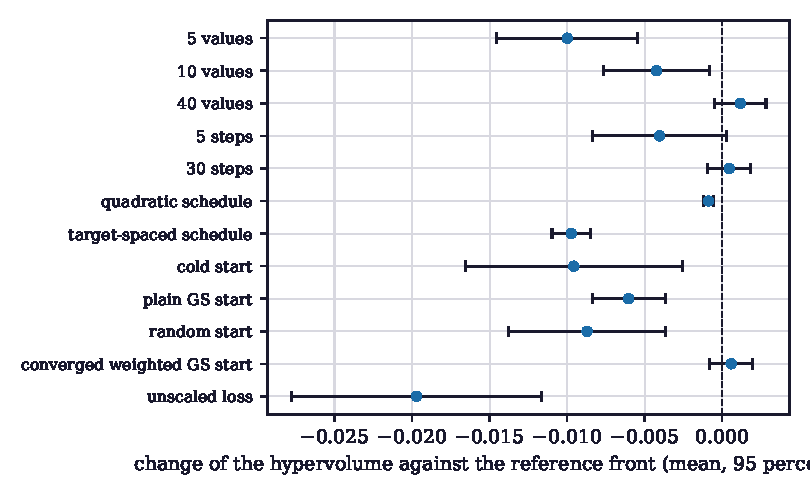
\includegraphics[width=0.84\textwidth]{fig-ablation.pdf}
\caption{Paired difference of the hypervolume of each variant from the reference front (points) with its 95 percent interval over \nSeedsAbl{} seeds (bars); variants are in the order of Table~\ref{tab:ablation}. Intervals that do not reach the dashed zero line are differences that five seeds distinguish from no change.}
\label{fig:ablation}
\end{figure}

\paragraph{The continuation.} A cold start, in which every weight begins from the refined start and not from its neighbour, lowers the hypervolume by \ablColdDiff{} (interval \ablColdDiffLo{} to \ablColdDiffHi), at the same cost. The efficiency that the cold front reaches at the largest weight is \ablColdEMax{} against \ablDefaultEMax{} for the warm front,
because fifteen steps from the start cannot travel as far as fifteen steps from a neighbour that has already travelled; and the number of its points that published iterates dominate rises from \ablDefaultDom{} to \ablColdDom{}. This is the measured form of Proposition~\ref{prop:warm}: the warm start spends its steps on a correction of the order of the step in the weight. The seventh hypothesis holds.
The same reading explains the two variants that vary the work per weight. With 5 steps per weight the hypervolume changes by \ablCgFiveDiff{} (interval \ablCgFiveDiffLo{} to \ablCgFiveDiffHi) and with 30 steps by \ablCgThirtyDiff{} (\ablCgThirtyDiffLo{} to \ablCgThirtyDiffHi); both intervals contain zero, so the default of 15 is on a plateau of the hypervolume, and the 30 steps cost \ablCgThirtySec{} seconds against \ablDefaultSec{}, nearly twice as much, for a change that five seeds do not distinguish from none.
The number of weights matters more at the low end: 5 weights lower the hypervolume by \ablNLamFiveDiff{} (\ablNLamFiveDiffLo{} to \ablNLamFiveDiffHi) and 10 weights by \ablNLamTenDiff{} (\ablNLamTenDiffLo{} to \ablNLamTenDiffHi), because the front is then a polygon with few vertices and the area under it is underestimated, while 40 weights change it by \ablNLamFortyDiff{} (\ablNLamFortyDiffLo{} to \ablNLamFortyDiffHi), again within the interval of no change, at \ablNLamFortySec{} seconds.
So the hypervolume is already resolved at 20 weights, and the number of points on the front is the only thing that more weights buy.

\paragraph{The start.} The front depends on the hologram from which it starts, because that hologram sets the total light $e_0$ of the target. Starting from 30 iterations of plain GS lowers the hypervolume by \ablStartGsDiff{} (\ablStartGsDiffLo{} to \ablStartGsDiffHi), starting from the random superposition with no iteration by \ablStartRandDiff{} (\ablStartRandDiffLo{} to \ablStartRandDiffHi), and both are distinguished from no change.
Starting from the hologram of weighted GS after 100 iterations, which has a higher efficiency than the phase-fixed start (the first point of the front has a mean efficiency of \ablStartGswHEFirst{} against \ablDefaultEFirst{}), changes the hypervolume by \ablStartGswHDiff{} (\ablStartGswHDiffLo{} to \ablStartGswHDiffHi), which is no change at this number of seeds, and removes the domination of the front by published iterates: the number of dominated points falls from \ablDefaultDom{} to \ablStartGswHDom{}. The choice of the start of the module is therefore sound for the hypervolume and is
not the best choice for the uniform end, where a better-converged start gives a better first part of the front at no cost in area.

\subsection{Schedule of the weights and scaling of the loss}\label{sec:abl-schedule}

\begin{figure}[t]
\centering
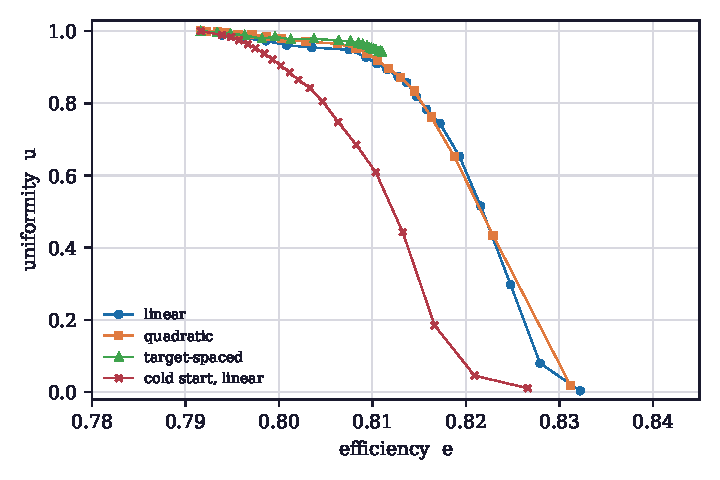
\includegraphics[width=0.78\textwidth]{fig-schedule.pdf}
\caption{Front of seed 1 for the linear schedule of the weights (blue circles), the quadratic schedule (orange squares), the target-spaced schedule of Proposition~\ref{prop:shift} (green triangles) and the cold start with the linear schedule (red crosses), on the ten by ten lattice. The target-spaced schedule covers the uniform end more finely and stops near the efficiency of 0.81; the cold start trails the others in efficiency at equal uniformity.}
\label{fig:schedule}
\end{figure}

The quadratic schedule, dense near the uniform end, changes the hypervolume by \ablQuadDiff{} (interval \ablQuadDiffLo{} to \ablQuadDiffHi); the interval excludes zero, and the size is a tenth of a percent, so the schedule is a second-order choice. The target-spaced schedule, the one that Proposition~\ref{prop:shift} suggests, lowers the hypervolume by \ablTargetDiff{} (\ablTargetDiffLo{} to \ablTargetDiffHi), and Figure~\ref{fig:schedule} shows why: it spaces its 20 points evenly in the total light that the target asks for,
from the efficiency of the start up to a total of one, which corresponds to weights up to \ablTargetLamMax{}; the front it returns stops at a largest efficiency of \ablTargetEMax{} and a lowest uniformity of \ablTargetUMin{}, and it omits the efficient tail that the linear schedule reaches (\ablDefaultEMax{} and \ablDefaultUMin{}). The schedule resolves the useful part of the front well, with uniformity above 0.94, and it is the better choice
when the useful part is the question; it gives a lower hypervolume because the criterion counts the tail, so the schedule is a matter of the purpose of the front. The prediction of the proposition that most points of a linear grid fall beyond $\lambda^\ast$ is correct, and the cost of it is small in area terms.

The scaling of the loss is the largest effect in the table. Without the two divisions the shift $\delta_\lambda$ of Proposition~\ref{prop:shift} is $\lambda/(2(1-\lambda))$ per trap, which is \rawFactor{} times (the factor $M/e_0$) the shift of the scaled loss at the same weight, so at the first weight after the origin, $\lambda=\ablRawLamOne{}$, the loss asks for a raise of every trap by \rawShiftRel{} times its intensity, and the front collapses: the mean uniformity at that weight is \ablRawFirstU{} and every later point has a uniformity of at most \ablRawLaterU{}; the hypervolume is lower by \ablRawDiff{} (\ablRawDiffLo{} to \ablRawDiffHi) and only \ablRawNPar{} of the points are non-dominated on average. The efficiency
at the efficient end is the same, \ablRawEMax{} against \ablDefaultEMax{}, so what the scaling buys is the middle of the front. The normalization is the reason that one weight means the same on every array, and this variant measures what its absence costs on the task.

\subsection{What each component contributes}\label{sec:abl-summary}

In the order of the size of the effect, the unscaled loss costs \ablRawDiff{}, the target-spaced schedule \ablTargetDiff{}, the cold start \ablColdDiff{}, the random start \ablStartRandDiff{}, the plain GS start \ablStartGsDiff{} and 5 weights \ablNLamFiveDiff{}, all lower than the reference and all excluded from zero by their intervals. The components that carry the front are therefore the normalization of the loss, the warm start along the weights and a start that is already close to uniform. The number of steps per weight and the number of weights above 20 are
on a plateau, and the converged start of weighted GS does not change the area. The surprising outcome is the start: the module's start is not the best start for the part of the front near the uniform end, which a front computed from weighted GS after 100 iterations covers without domination, and the area is the same.
Two further readings follow from the table. The seconds of the variants follow the number of weights and of steps, as the cost model of Section~\ref{sec:complexity} says, and the start from weighted GS after 100 iterations is the cheapest of the full-length variants, \ablStartGswHSec{} seconds against \ablDefaultSec{}.
And the lowest uniformity of the variants that reach $\lambda=1$ lies between \ablRawUMin{} (unscaled loss) and \ablCgFiveUMin{} (5 steps per weight), against \ablTargetUMin{} for the target-spaced schedule that stops earlier, so the tail of the front is set by the weight and its depth by the steps.
